% Matteo Veneziano -- Solid State Physics Formula Sheet
\graysec{Réseaux cristallins dans l'éspace réel et réciproque}
\begin{squishlist}
    \item DIFFERENTES LIAISONS
\end{squishlist}
\graypar{Réseaux cristallins}
\begin{squishlist}
    \item $\vec{R} = \sum_{j=1}^{3} n_j \vec{a}_j$ un vecteur du \textbf{réseau de Bravais (RB)} (réseau de points)
    \item Une \textbf{cellulle (ou maille) primitve} est un volume d'espace qui, translaté par les vecteurs $\vR$ du RB, remplit exactement l'espace sans recouvrement. Ne contient qu'un point du RB, donc a volume $v = 1/n$ avec $n$ la densité de points du RB.
    \item La \textbf{cellule de Wigner-Seitz} est la région de l'espace qui est plus proche à un point du RB que de n'importe quel autre point. On l'obtient en tracant les plans bissecteurs des ligne qui connectent les points.
    \item Une \textbf{structure cristalline} est un RB avec une base formée de un ou plus atomes
    \begin{minipage}{.25\columnwidth}
        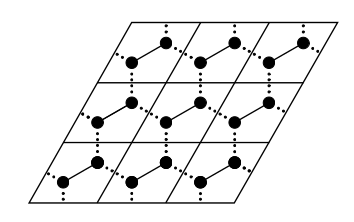
\includegraphics[width=2cm]{figures/abeille.png}
    \end{minipage}
    \begin{minipage}{.75\columnwidth}
        E.g.: réseau nid d'abeille du graphène dérive d'un RB hexagonal avec base de deux atomes
    \end{minipage}
    \item Le \textbf{réseau réciproque} est formée des $\vG$ t.q.\ $\exp(i \vG \cdot \vR) = 1$ \\
    $\vG = \sum_{i=1}^{3}h_i \vec{b}_i $\squishsep $\vec{a}_i \cdot \vec{b}_j = 2 \pi \delta_{ij}$ \squishsep $\vec{b}_1 = 2 \pi \frac{\vec{a}_2 \times \vec{a}_3}{\vec{a}_1 \cdot (\vec{a_2 \times \vec{a}_3})}$ et perm.\ cycl.\
\end{squishlist}    
\graypar{boh}
\begin{squishlist}
    \item Conditions de Born-von-Karman: $\psi(\vec{r} + N_j \vec{a}_j) = \psi(\vec{r}), \, \forall j=1,2,3$ où $\vec{a}_j$ est un vecteur primitif du réseau de Bravais, $N_j$ un entier positif.
    \item $N$ valeurs $\vec{k}$ admises dans chaque zone de Brillouin $\rightarrow$ $2N$ états électroniques (spin)
    \item Densité électronique $n = \frac{N}{V} = \int_0^{E_F} g(E) \ud E$
\end{squishlist}

\graypar{Surface de Fermi}
\begin{squishlist}
    \item Trouver $k_F$: vol. sphère de Fermi $\Omega_F$ $\times$ densité de $k$ $\times \; 2$ (spin) = \# $e^-$ dans système 
    \item $E_F = \frac{\hbar^2 k_F^2}{2m}$
\end{squishlist}

\graysec{Électrons libres}
\begin{squishlist}
    \item Densité d'états $g(E)$ HOW IS IT FOUND
    \item Distribution de Fermi-Dirac $f(E,T) = \frac{1}{\exp\left(\frac{(E- \mu)}{k_B T}\right) + 1}$
    \item Potentiel chimique $\mu(T) = E_F - \frac{\pi^2}{6}(k_B T)^2 \frac{1}{g(E_F)} \left.\dder{g}{E}\right|_{E_F}$
    \item Chaleur specifique $c_V = \frac{\pi^2}{3}K_B^2 T \, g(E_F) $
    \item $\chi_{\text{Pauli}}$ FILL
    \item $\tau$ FILL
    \item Conductivité électrique $\sigma = \frac{n e^2 \tau(E_F)}{m}$ diminue avec $T$ (parce que $\tau$ diminue avec $T$)
    \item Conductivité thermique $\kappa = \frac{1}{3}V_F^2 \tau(E_F) c_V$
    \item Loi de Wiedemann-Franz: $\frac{\kappa}{\sigma T} = \frac{\pi^2}{3}\left(\frac{k_B}{e}\right)$
\end{squishlist}

\graysec{Les électrons dans un potentiel périodique. Structure de bande}
\graypar{Théorème de Bloch}
\begin{squishlist}
    \item $\psi(\vec{r} + \vec{R}) = \exp(i\vec{k} \cdot \vec{R}) \psi(\vec{r})$
    \item Un vecteur $\vec{k}$ ne se trouvant pas dans la 1ZDB peut être réduit à la 1ZDB: $\tilde{\vec{k}} = \vec{k} + \vec{G}$ \\
    car $\vec{k}$ est défini à un vecteur du réseau réciproque près, i.e. $\exp(i \vec{G}\cdot \vec{R}) = 1$.
    \item Alternative: $\psi_{n \vec{k}}(\vr) = \exp(i \vk \cdot \vr ) u_{n \vk}(\vr)$ où $u_{n \vk}(\vr) =  u_{n \vk}(\vr+ \vR)$
\end{squishlist}

\graypar{Équation centrale}
\begin{squishlist}
    \item On peut décomposer une fonction d'onde $\psi(\vr)$ qui satisfait Born-von-Karman comme $\psi(\vr) = \sum_{\vk} a_{\vk} \exp(i \vk \cdot \vr)$
    \squishsep $\psi_{n,\tilde{\vk}} = \sum_{\vG} a_{n, \tilde{\vk}-\vG} \exp(i (\tilde{\vk} - \vG) \cdot \vr) \quad n=1\rightarrow\infty$
    \item Le potentiel a la périodicité du réseau: $U(\vr) = \sum_{\vG} U_{\vG} \exp(i \vG \cdot \vr)$
    \item $\left(\frac{\hbar^2 k^2}{2m} - E\right)a_{\vk} + \sum_{\vG}U_{\vG}a_{\vk - \vG}  = 0$
    \item $(E_{\vk}^0 - E)a_{\mathbf{{\tilde{k}}} - \vG} + \sum_{\vG'}U_{\vG' - \vG}a_{\mathbf{\tilde{k}} - \vG'}  = 0$
    \item Periodicité de l'énergie $ E_{n,\mathbf{\tilde{k}} + \vG} = E_{n,\mathbf{\tilde{k}}}$
    \item Électrons libres: $U(\vr) = 0 \Longrightarrow E_{k - G_i}^0 = \frac{\hbar^2(k - G_i)^2}{2m}$
\end{squishlist}

\graypar{Modèle des électrons faiblement couplés au réseau (quasi-libres)}
Part de l'approximation du gaz d'électrons libres et suppose une corrugation faible du potentiel, due au fait que: 
1) les interactions sont fortes surtout à courtes distances et le principe d'exclusion de Pauli empêche les électrons de conduction de pénétrer dans le coeur et 
2) les électrons de coeur écrantent le noyau positif. Ce modèle s'applique en général bien aux électrons de valence de type s - p, donc pour les alcalins (groupe I), alcalins terreux (groupe II), métaux nobles.
\begin{squishlist}
    \item États presque dégénérés: $(E_{k-G_i}^0 - E) c_{k-G_i} + \sum_{j=1}^m U_{G_j - G_i} c_{k-G_j} = 0$ \\
    $i,j = 1 \ldots m$ tels que $|E_{k-G_i}^0 - E_{k-G_j}^0| \lesssim U$, \quad $U_G$ coefficients de Fourier de $U$. \\
    Peut être mis sous forme matricielle, trouver energies propres et vecteurs propres \\
    Levée de la dégénérescence $\rightarrow$ bandes d'énergies interdites.
    L’apparition d’un ”gap” d’énergie est donc reliée à la réflexion des fonctions d’onde électroniques (ondes planes) en bord de zone, qui crée des ondes
    stationnaires de densité de probabilité en $\cos^2$ ou $\sin^2$.
\end{squishlist}

\graypar{Modèle des liaisons fortes}
Part d'atomes neutres que l'on approche de plus en plus.
Les orbitales les plus étendues spatialement vont alors se recouvrir. Dans l'approximation
des liaisons fortes, on suppose que la fonction d'onde est bien décrite par les orbitales
atomiques, et on pose $H = H_{\text{at}} + \Delta U$. 
Cette approximation s'applique particulièrement
bien aux métaux de transition et aux isolants, qui ont un recouvrement d'orbitales pas
trop important.
\begin{squishlist}
    \item $E(\vk) = E + \frac{\beta + \sum_{\vR \neq 0}\exp(i\vk \cdot \vR) \; \gamma(\vR)}{1 + \sum_{\vR \neq 0}\exp(i\vk \cdot \vR)\; \alpha(\vR)}$
    $\left\{ \begin{aligned}
        & \alpha(\vR) = \int \phi^*(\vr)\phi(\vr - \vR) \ud^3 r \\
        & \beta = \int \phi^*(\vr)\Delta U (\vr) \phi(\vr) \ud^3 r \\
        & \gamma(\vR) = \int \phi^*(\vr)\Delta U (\vr) \phi(\vr - \vR) \ud^3 r
    \end{aligned} \right.$
    \item $\alpha(\vr)$ est positive pour fonction d'onde de type $s$, typiquement entre 0.1 et 0.4
    \item L'intégrale de champ cristallin $\beta < 0$ décrit l'effet du potentiel généré par les autres atomes.
    \item L'intégrale de transfert $\gamma(R)$ décrit le passage d'un électron du site initial $R = 0$ au site $R$, induit par la présence du potentiel $\Delta U$.
\end{squishlist}

\graypar{Métaux, isolants, semiconducteurs}
$2N$ fonctions de Bloch indépendantes dans chaque zone de Brillouin.
À chaque zone de Brillouin on peut associer une bande d'énergie qui peut donc "contenir" $2N$ électrons.
S’il y a un seul électron de valence par cellule primitive, la bande d’énergie
est à moitié remplie par les électrons.
\begin{squishlist}
    \item  nb $e^-$ par maille \textbf{impair}: forcement \textbf{métal}
    \item  nb $e^-$ par maille \textbf{pair}: \textbf{métal} si les bandes d'énergie se recouvrent (deux bandes partiellement remplies); \textbf{isolants} si elles ne se recouvrent pas (électrons remplissent enti`erement une bande d’énergie, les autres bandes étant vides) ou \textbf{semiconducteurs} si la largeur de la bande interdite est faible ($\sim 1 $ eV) (il est possible de faire passer par excitation thermique des électrons de la bande pleine à la vide, conductibilité électrique qui croît lorsque la température augmente).
    \item Metaux de transition ont plus grande $g(E_F)$ $E_F$ est sur bande $d$ qui a densité d'état plus élevée.
\end{squishlist}


\graysec{Dynamique des électrons}
\begin{squishlist}
    \item Équations du mouvement entre collisions, $n$ constante du mouvem.
    $ \left\{ \begin{aligned} 
        & \dot{\vec{r}} = \vec{v_n}(\vk) = \frac{1}{\hbar} \vec{\nabla_\vec{k}E_n}(\vk) \\
        & \hbar \dot{\vec{k}} =  -e (\vec{E} + \vec{v_n}(\vk) \times \vec{B}) =  -e (\vec{E} + \frac{1}{\hbar} \vec{\nabla_\vec{k}E_n}(\vk) \times \vec{B})
    \end{aligned} \right. $
    
    \item Pour un $e^-$ de Bloch (potentiel non-nul) $\hbar \vk \neq \vec{p}$
    \item Une bande pleine de conduit pas: \\
    $\vec{j} = -e \int_{\text{zone Brillouin}} \frac{\ud^3 k}{4 \pi^3}\vec{v} = -e \frac{1}{\hbar} \int_{\text{zone Brillouin}} \frac{\ud^3 k}{4 \pi^3} \D{\vec{k}}{E} = 0$ \\
    car pour toute fonction périodique $f(\vk) = f(\vk + \vG)$ on a $\int_{\text{cell.\ prim.}}\ud^3 k \D{\vk}{f(\vk)} = 0$
    \item Sous l’effet du champ $E$ le remplissage
    des états par les électrons n’est pas modifié, car deux états électroniques de la même bande qui diffèrent d’un vecteur du réseau réciproque doivent être considérés comme le même état.
    \item Concept de \textbf{trou}: $\vec{j} = -e \int_{\text{états occupés}} \frac{\ud^3 k}{4 \pi^3}\vec{v} = +e \int_{\text{états vides}} \frac{\ud^3 k}{4 \pi^3}\vec{v}$
    \item Niveau électron.\ \textbf{proche du sommet d'une bande}: $E(\vk) = E(\vk_0) - A(\vk - \vk_0)^2$ \\
    On définit la masse effective $m^*$ par $A = \frac{\hbar^2}{2m^*}$.
    Un trou se comporte au voisinage du sommet d’une bande
    comme une particule de charge $+e$ et de masse $m^*$. Trous lourds ont paraboles larges, trous légers ont paraboles étroites.

    \item Dans l’espace réciproque les trajectoires électroniques sont situées à l’intersection d’une surface d’énergie constante et d’un plan perpendiculaire à $B$.
    \begin{itemize}
        \item $\nabla E(\vk)$ pointe vers l'éxter.\ de la surf.\ $E(\vk) = $ cte $\Rightarrow$ trajectoire électronique
        \item $\nabla E(\vk)$ pointe vers l'inter.\ de la surf.\ $E(\vk) = $ cte $\Rightarrow$ trajectoire de type trou
    \end{itemize}
\end{squishlist}

\graysec{Les semiconducteurs}
Un semiconducteur est intrinsèque si ses proprietés électroniques sont dominées par les $e^-$ excités thermiquement de la bande de valence à la bande de conduction et extrinsèque si elles sont dominées par les $e^-$ contribués à la bande de conduction ou capturé par la bande de valence par des impuretés.
\begin{squishlist}
    \item Densité d'$e^-$ dans bande de conduction $n(T) = \int_{E_c}^{\infty} g_c(E) \frac{1}{e^{(E-\mu)/k_B T} + 1} \ud E$
    \item Densité de trous dans bande de valence $p(T) =\int_{E_c}^{\infty} g_v(E)\left( 1- \frac{1}{e^{(E-\mu)/k_B T} + 1} \right)\ud E$
    \item Pour un sc non dégénéré ($E_c - \mu \gg k_B T, \mu -E_v \gg k_B T)$ on a \\ $n(T) = N(T) e^{-(E_c - \mu) / k_B T}$ \quad $p(T) = P(T) e^{-(\mu - E_v) / k_B T}$
    \item Bande quadratique: $g_{c,v}(E) = \frac{1}{2 \pi^2}\left( \frac{2m^*_{c,v}}{\hbar^2}\right) \sqrt{E - E_{c,v}}$
    d'où \\
    $N(T) = \frac{1}{4} \left( \frac{2 m_c^* k_B T}{\pi \hbar^2}\right)^{3/2}=2.5 \left(\frac{m_c^*}{m}\right)^{3/2} \left(\frac{T}{300 \mathrm{K}}\right)^{3/2} 10^{19}/\mathrm{cm}^3; \quad P(T) = \frac{1}{4} \left( \frac{2 m_v^* k_B T}{\pi \hbar^2}\right)^{3/2}$
    \item \textbf{Loi d'action de masse:} $n(T)p(T) = N(T)P(T) e^{-\beta E_g}$
    \item sc \textbf{intrinsèque} $n(T) = p(T) = n_i(T)$ \quad densité d'$e^-$ excités thermiquement \\
    $\Longrightarrow n_i(T) = \sqrt{n(T) p(T)} = e^{-E_g / 2 k_B T} \sqrt{N(T) P(T)}$ \\
    $\Longrightarrow \mu_i(T) = E_v + \frac{1}{2}E_g + \frac{1}{2}k_B T \ln \left( \frac{P(T)}{N(T)}\right) = E_v + \frac{1}{2}E_g + \frac{3}{2}\frac{1}{2}k_B T \ln \left( \frac{m_v^*}{m_c^*}\right)$
\end{squishlist}

\graypar{Semiconducteur dopé}
Ajout d’impuretés à un SC.
L’impureté doit avoir un nombre d’électrons de valence différent de celui du SC pur. Si la valence de l’impureté est supérieure à celle du SC, nous sommes en présence d’un \textbf{donneur} (l’impureté “donne” un électron au semi-conducteur), tandis que si la valence est inférieure, nous sommes en présence d’un \textbf{accepteur} (l’impureté "prend" un électron au SC, autrement dit, lui "donne" un trou)
\begin{squishlist}
    \item Impuretés modèlisées avec atome d'H avec corrections: masse effective $m^*$ et constante diélectrique $\varepsilon_r$ du SC 
    $\Longrightarrow r_0 = \frac{\varepsilon_r}{m^*/m} a_0; \quad E=\frac{m^*/m}{\varepsilon_r^2}E_H$
    \item $n = \frac{1}{2}\sqrt{\Delta n^2 + 4 n_i^2} + \frac{1}{2}\Delta n;\quad \Delta n = n - p$
    \item $\frac{\Delta n }{n_i} = \frac{n-p}{\sqrt{np}} = 2 \sinh (\beta(\mu - \mu_i))$
    \item $\sigma = n e \nu_e + p e \nu_h$
\end{squishlist}    

\graypar{Jonction pn}
En polaris.\ directe le courant est dû aux porteurs majoritaires (\elec qui provienn,\ de la region $n$ et trous de la region $p$) par diffusion et recombinaison.
En polaris.\ inverse le courant est dû aux porteurs minoritaires générés thermiquement, favoris par champ électrique.